%to have line numbers
%\RequirePackage{lineno}
\documentclass[10pt, letterpaper]{article}      
\usepackage[margin=.1cm,font=small,labelfont=bf]{caption}[2007/03/09]
%\usepackage{endnotes}
\usepackage{setspace}
\usepackage{longtable}                        
\usepackage{anysize}                          
\usepackage{natbib}                           
%\bibpunct{(}{)}{,}{a}{,}{,}                   
\bibpunct{(}{)}{,}{a}{}{,}                   
\usepackage{amsmath}
\usepackage[pdftex]{graphicx}                
\usepackage{epstopdf}
\usepackage{hyperref}                             % For creating hyperlinks in cross references


% \usepackage[margins]{trackchanges}

% \note[editor]{The note}
% \annote[editor]{Text to annotate}{The note}
%    \add[editor]{Text to add}
% \remove[editor]{Text to remove}
% \change[editor]{Text to remove}{Text to add}



\marginsize{1cm}{1cm}{.5cm}{.5cm}%{left}{right}{top}{bottom}   
					          % Helps LaTeX put figures where YOU want
 \renewcommand{\topfraction}{1}	                  % 90% of page top can be a float
 \renewcommand{\bottomfraction}{1}	          % 90% of page bottom can be a float
 \renewcommand{\textfraction}{0.0}	          % only 10% of page must to be text

 \usepackage{float}                               %latex will not complain to include float after float

\usepackage[table]{xcolor}                        %for table shading
\definecolor{gray90}{gray}{0.90}
\definecolor{orange}{RGB}{255,128,0}

\renewcommand\arraystretch{.9}                    %for spacing of arrays like tabular

%-------------------- my commands -----------------------------------------
\newenvironment{ig}[1]{
\begin{center}
 %\includegraphics[height=5.0in]{#1} 
 \includegraphics[height=3.3in]{#1}
\end{center}}

 \newcommand{\cc}[1]{
\hspace{-.13in}$\bullet$\marginpar{\begin{spacing}{.6}\begin{footnotesize}{#1}\end{footnotesize}\end{spacing}}
\hspace{-.13in} }

%-------------------- END my commands -----------------------------------------



%-------------------- extra options -----------------------------------------

%%%%%%%%%%%%%
% footnotes %
%%%%%%%%%%%%%

%\long\def\symbolfootnote[#1]#2{\begingroup% %these can be used to make footnote  nonnumeric asterick, dagger etc
%\def\thefootnote{\fnsymbol{footnote}}\footnote[#1]{#2}\endgroup}	%see: http://help-csli.stanford.edu/tex/latex-footnotes.shtml

%%%%%%%%%%%
% spacing %
%%%%%%%%%%%

% \abovecaptionskip: space above caption
% \belowcaptionskip: space below caption
%\oddsidemargin 0cm
%\evensidemargin 0cm

%%%%%%%%%
% style %
%%%%%%%%%

%\pagestyle{myheadings}         % Option to put page headers
                               % Needed \documentclass[a4paper,twoside]{article}
%\markboth{{\small\it Politics and Life Satisfaction }}
%{{\small\it Adam Okulicz-Kozaryn} }

%\headsep 1.5cm
% \pagestyle{empty}			% no page numbers
% \parindent  15.mm			% indent paragraph by this much
% \parskip     2.mm			% space between paragraphs
% \mathindent 20.mm			% indent math equations by this much

%%%%%%%%%%%%%%%%%%
% extra packages %
%%%%%%%%%%%%%%%%%%

\usepackage{datetime}


\usepackage[latin1]{inputenc}
\usepackage{tikz}
\usetikzlibrary{shapes,arrows,backgrounds}


%\usepackage{color}					% For creating coloured text and background
%\usepackage{float}
\usepackage{subfig}                                     % for combined figures

\renewcommand{\ss}[1]{{\colorbox{blue}{\bf \color{white}{#1}}}}
\newcommand{\ee}[1]{\endnote{\vspace{-.10in}\begin{spacing}{1.0}{\normalsize #1}\end{spacing}\vspace{.20in}}}




\usepackage{sectsty}
\allsectionsfont{\normalfont\sffamily}



\usepackage{sectsty}
\allsectionsfont{\normalfont\sffamily}
\usepackage[margins]{trackchanges}

\renewcommand\familydefault{\sfdefault}

\usepackage{verbatim}
\usepackage{rotating}
\usepackage{catchfilebetweentags}
%-------------------- END extra options -----------------------------------------
\date{Draft: {}\today}
\title{Graphs and Tables and SOM: Supplementray Online Material for paper
}
\author{
Adam Okulicz-Kozaryn\thanks{EMAIL: adam.okulicz.kozaryn@gmail.com
  \hfill I thank XXX.  All mistakes are mine.} \\
{\small Rutgers - Camden}\\
Micah Altman\thanks{EMAIL: ???
  \hfill I ???} \\
{\small MIT}
}

\begin{document}

%%\setpagewiselinenumbers
%\modulolinenumbers[1]
%\linenumbers

\bibliographystyle{/home/aok/papers/root/tex/ecta}
\maketitle
\vspace{-.4in}
\begin{center}
\end{center}

\begin{spacing}{1.4}

\tableofcontents


\section{PAPER Tables and Graphs}


\textbf{TODO grpahs and tables for paper body here}


\newpage
\section{\huge Only ONLINE APPENDIX}
\textbf{[note: this section will NOT be a part of the final version of
  the manuscript, but will be available online instead]} %hence everything belowis organized by section, not subsection


!!!TODO look more carefully at energy definitions!!

\section{General Considerations}

\subsection{Electricty use: residential and non-residential} 
How is electricity used in United States homes? This is an important
consideration because it really shows what we do with this electricity--how we
consume it, what are the end uses. Data are shown in table
\ref{eleEndUse}. Furthermore end uses of energy changed over time, for instance
 from 1993 to 2009: applianes share increased from 24\% to 35\% and space
 heating dropped from 53\% to 41\%
 \url{http://www.eia.gov/todayinenergy/detail.cfm?id=10271&src=%E2%80%B9%20Consumption%20%20%20%20%20%20Residential%20Energy%20Consumption%20Survey%20%28RECS%29-b1}. 
Also, the good news is that average energy consumption per household dropped from 114 m BTU in 1980 to
90 m BTU in 2009 \url{http://www.eia.gov/consumption/residential/reports/2009/consumption-down.cfm?src=%E2%80%B9%20Consumption%20%20%20%20%20%20Residential%20Energy%20Consumption%20Survey%20%28RECS%29-b5}.  


\begin{table}[H]\centering\footnotesize
\caption{\label{eleEndUse}  Estimated U.S. Residential Electricity Consumption by End
  Use, 2012 \url{www.eia.gov/tools/faqs/faq.cfm?id=96&t=3}}
\begin{tabular} {llll}   \hline 
End Use&Quadrillion\\\hline 
Btu &Billion\\
kilowatthours &Share of\\
total \\
Space cooling&0.85&250&18.00\%\\
Lighting&0.64&186&14.00\%\\
Water heating&0.45&130&9.00\%\\
Refrigeration&0.38&111&8.00\%\\
Televisions and related equipment 1&0.33&98&7.00\%\\
Space heating&0.29&84&6.00\%\\
Clothes dryers&0.2&59&4.00\%\\
Computers and related equipment2&0.12&37&3.00\%\\
Cooking&0.11&31&2.00\%\\
Dishwashers3 &0.1&29&2.00\%\\
Furnace fans and boiler circulation pumps&0.09&28&2.00\%\\
Freezers&0.08&24&2.00\%\\
Clothes washers3&0.03&9&1.00\%\\
Other uses4&1.02&299&22.00\%\\
Total consumption&4.69&1375&\\\hline
\end{tabular}\end{table}


\subsection{TODO Petroleum use: residential and non-residential} 
\subsection{TODO Natural Gas use: residential and non-residential} 

\section{countries}

Literature about happiness across countries usually focuses on role of income,
with a well known Easterlin Paradox, where economic growth does not lead to
greater happiness over time.\footnote{veenhoven's criticsim--have it
somewhere--easterlin delusion etc}. Yet, in space, across countries it is agreed
upon that richer countries are happier at least with quadratic relationship. 

In this study we aregue that countries that consumer more enrgy are not happier
when controlling for income--and interpret this as another argument for energy
conservation. Also it counters commoin wisodom--one could think that greater
energy consumption leasd to greater happiness--if not then whatt;s the point of
energy consumption. 

One explanation is that sustainable people are happy (cite that i think
ecological economics paper--shoudl be in ebib)


\subsection{europe-mannheim}

\ig{/tmp/ls_en/couLsEne.pdf}

\ig{/tmp/ls_en/couLsGdp.pdf}

\subsection{world}

\ig{/tmp/ls_en/couWvsLsEne.pdf}

\ig{/tmp/ls_en/couWvsLsGdp.pdf}

very interesting--when controlling fpr gdp, energy becomes negativbe!!
\ig{/tmp/ls_en/couWvsLsEnGdp.pdf}



\section{Census Divisions}

\begin{figure}[H]
 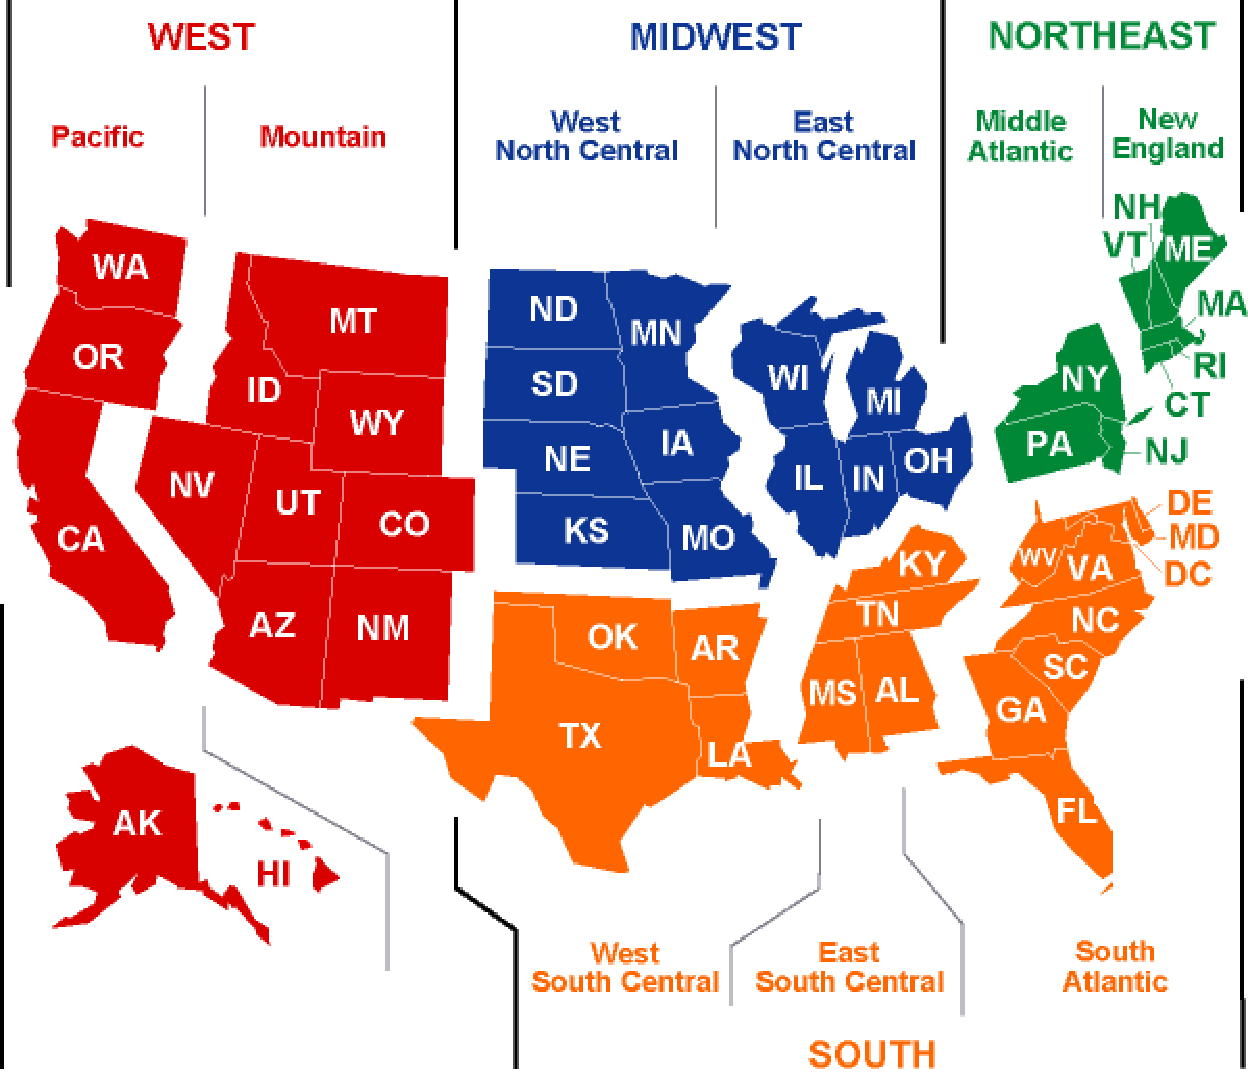
\includegraphics[height=3in]{/home/aok/papers/lonnie_issp_work/tex/cendivco.pdf}\centering
\caption{Census divisions.}\label{cenDiv}
\end{figure}

have a ts graph here showing happiness by division and lectricity
consumption--guess smooth them

\section{States}

This paper started as one author frequently flies from NJ to TX and noticed from
the air and on the ground huge differences in energy use between the two
states. Bigger houses, roads, cars, indeed everything is big in Texas! And
indeed differences are striking--Texas consumee about twice as much enbrgy as NJ
does per capita; yet interestingly not a big difference in residential energy
consumption--perhaps everything is newer in TX and hence more enrgy
efficent. The biggest diffences are in transportation ?? v ?? -->>


\begin{spacing}{.8}
{\footnotesize
\begin{verbatim}
TETPB    Total energy consumption per capita, m BTU
TERPB    Total energy consumption per capita in the residential sector, m BTU
TEAPB    Total energy consumption per capita in the transportation sector, m BTU
TECPB    Total energy consumption per capita in the commercial sector, m BTU
TEIPB    Total energy consumption per capita in the industrial sector, m BTU

sorted on TETPB, this is for 2009

. | state   TETPB   TERPB   TEAPB   TECPB   TEIPB |
  |-----------------------------------------------|
  |    RI     182      58      60      44      20 |
  |    NY     192      56      56      62      18 |
  |    HI     205      27     100      31      48 |
  |    MA     211      65      69      42      35 |
  |    CA     212      40      84      41      47 |
  |-----------------------------------------------|
  |    CT     215      71      68      52      23 |
  |    AZ     219      59      76      52      31 |
  |    FL     222      66      77      54      25 |
  |    NH     227      69      80      51      27 |
  |    NV     244      58      80      43      63 |
  |-----------------------------------------------|
  |    VT     248      80      85      47      36 |
  |    MD     256      74      81      74      27 |
  |    OR     269      68      87      51      63 |
  |    NC     273      78      76      63      56 |
  |    NJ     273      68     103      72      31 |
  |-----------------------------------------------|
  |    MI     274      76      75      61      62 |
  |    UT     274      59      86      55      74 |
  |    PA     287      73      77      54      83 |
  |    DE     294      77      79      71      67 |
  |    CO     296      68      85      60      83 |
  |-----------------------------------------------|
  |    IL     303      76      78      63      86 |
  |    GA     304      76      98      57      73 |
  |    WA     307      77      91      59      80 |
  |    VA     308      81      93      78      56 |
  |    ME     311      68      94      48     101 |
  |-----------------------------------------------|
  |    WI     313      76      76      63      98 |
  |    MO     313      89      96      69      59 |
  |    OH     321      81      82      61      98 |
  |    DC     324      61      34     222       7 |
  |    NM     325      57      99      59     110 |
  |-----------------------------------------------|
  |    ID     326      82      80      55     109 |
  |    TN     333      84      96      60      93 |
  |    MN     340      77      90      66     108 |
  |    SC     345      79      99      57     110 |
  |    AR     360      78     100      57     125 |
  |-----------------------------------------------|
  |    MS     379      75     122      54     128 |
  |    WV     382      94      92      60     136 |
  |    AL     384      78      98      54     153 |
  |    KS     402      84     102      75     141 |
  |    OK     403      80     121      65     137 |
  |-----------------------------------------------|
  |    IN     423      87      92      59     186 |
  |    NE     431      88      99      77     168 |
  |    MT     431      90     116      81     144 |
  |    KY     449      89     110      60     191 |
  |    TX     452      64     110      58     219 |
  |-----------------------------------------------|
  |    SD     453      90     113      77     173 |
  |    IA     477      81     100      68     227 |
  |    ND     656     103     133      98     321 |
  |    LA     841      79     150      62     550 |
  |    AK     904      77     273      89     465 |
  |-----------------------------------------------|
  |    WY     933      85     217     111     519 |
  +-----------------------------------------------+

(obs=306)

             |    TERPB    TEAPB    TECPB    TEIPB    TETPB
-------------+---------------------------------------------
       TERPB |   1.0000
       TEAPB |   0.2141   1.0000
       TECPB |   0.2132   0.1255   1.0000
       TEIPB |   0.3914   0.7993   0.1818   1.0000
       TETPB |   0.4418   0.8620   0.3274   0.9757   1.0000


(obs=306)

             |    TERPB    TEAPB    TECPB    TEIPB    TETPB       ls
-------------+------------------------------------------------------
       TERPB |   1.0000
       TEAPB |   0.2141   1.0000
       TECPB |   0.2132   0.1255   1.0000
       TEIPB |   0.3914   0.7993   0.1818   1.0000
       TETPB |   0.4418   0.8620   0.3274   0.9757   1.0000
          ls |   0.0952   0.2740   0.1246   0.2629   0.2839   1.0000

ls is happiness
\end{verbatim}
}
\end{spacing}

Furthermore, interestingly transportation corrlates negatively with commerce--DC
one of the most effiicnet in trasportation (61) is least efficient in commerce
(222).  Total energy consumption correlates most with transportation (.86) and
 especially industry (.9). Happiness does correlate positively with all energy
 uses, mostly with transport and industry and total (about .3). 
  

\begin{figure}[H]
 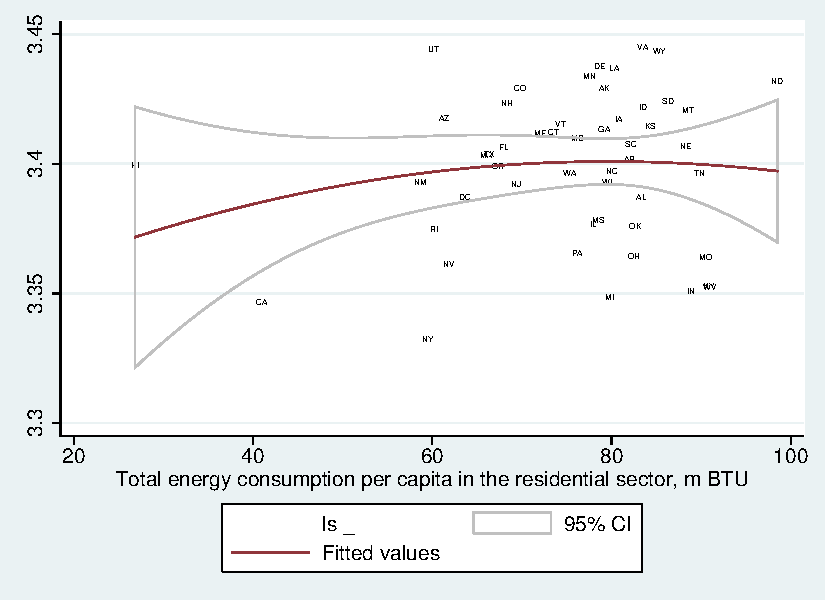
\includegraphics[height=3in]{/tmp/ls_en/lfTERPBls.pdf}\centering
\caption{lfTERPBls}\label{lfTERPBls}
\end{figure}

\begin{figure}[H]
 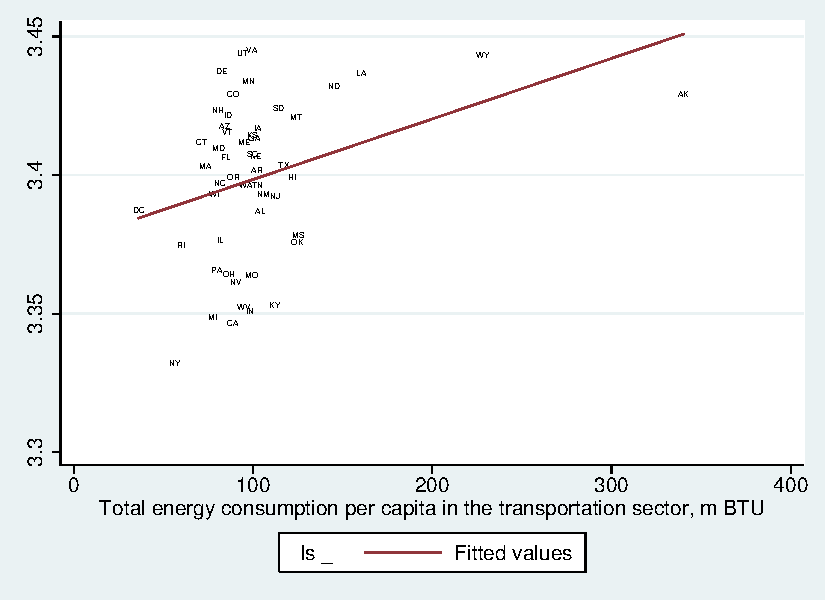
\includegraphics[height=3in]{/tmp/ls_en/lfTEAPBls.pdf}\centering
\caption{lfTEAPBls}\label{lfTEAPBls}
\end{figure}

\begin{figure}[H]
 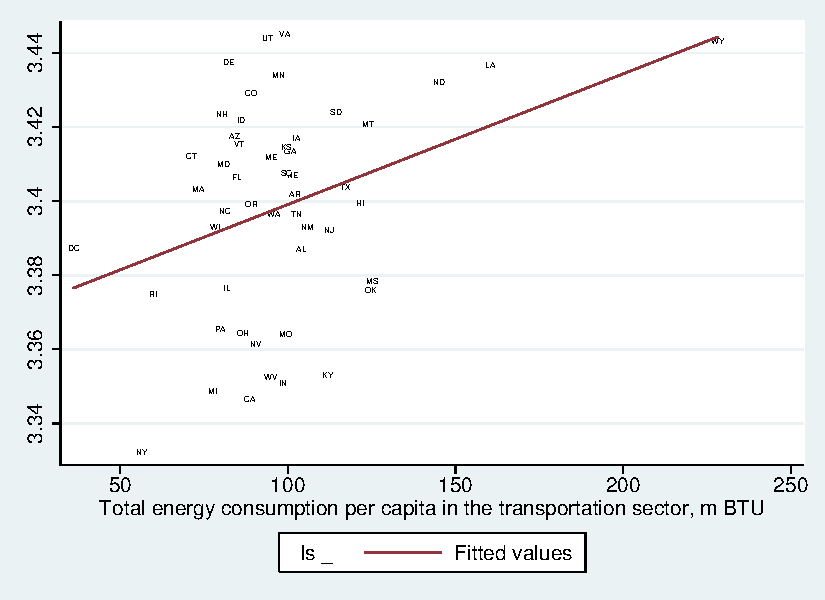
\includegraphics[height=3in]{/tmp/ls_en/lfTEAPBlsNoAk.pdf}\centering
\caption{no alaska; lfTEAPBlsNoAk}\label{lfTEAPBlsNoAk}
\end{figure}

\begin{figure}[H]
 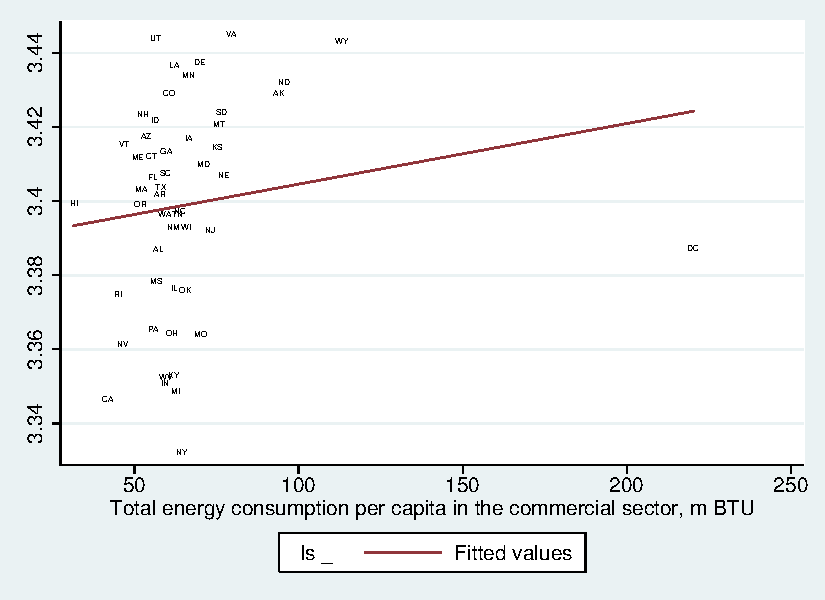
\includegraphics[height=3in]{/tmp/ls_en/lfTECPBls.pdf}\centering
\caption{lfTECPBls}\label{lfTECPBls}
\end{figure}

\begin{figure}[H]
 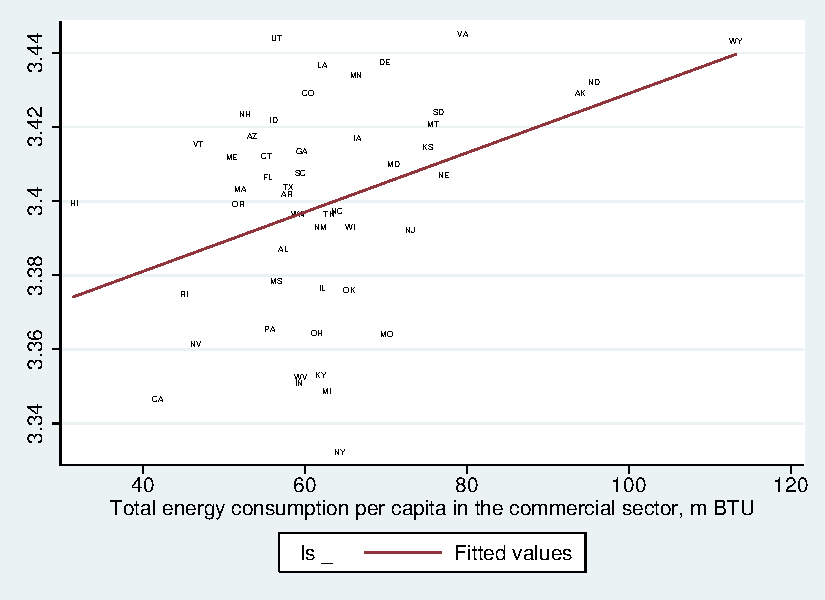
\includegraphics[height=3in]{/tmp/ls_en/lfTECPBlsNoDc.pdf}\centering
\caption{lfTECPBlsNoDc}\label{lfTECPBlsNoDc}
\end{figure}

\begin{figure}[H]
 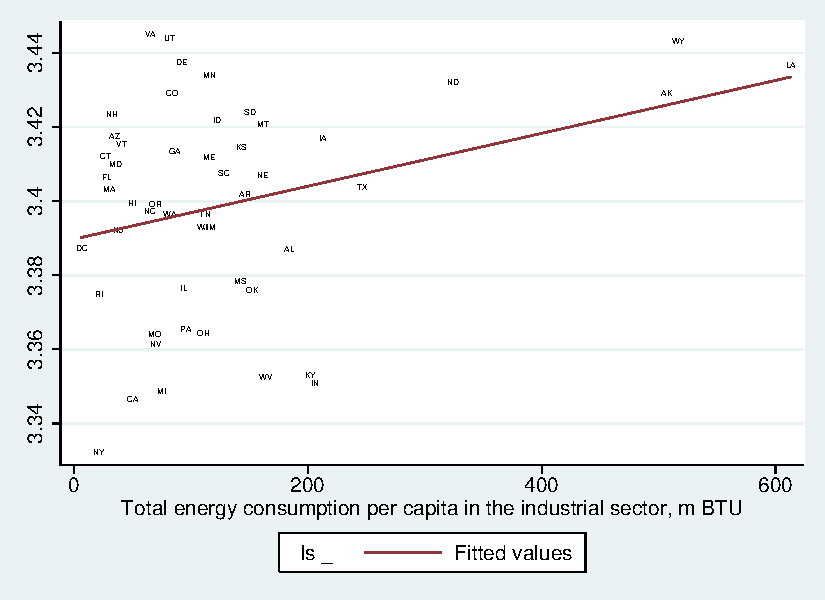
\includegraphics[height=3in]{/tmp/ls_en/lfTEIPBls.pdf}\centering
\caption{lfTEIPBls}\label{lfTEIPBls}
\end{figure}

\begin{figure}[H]
 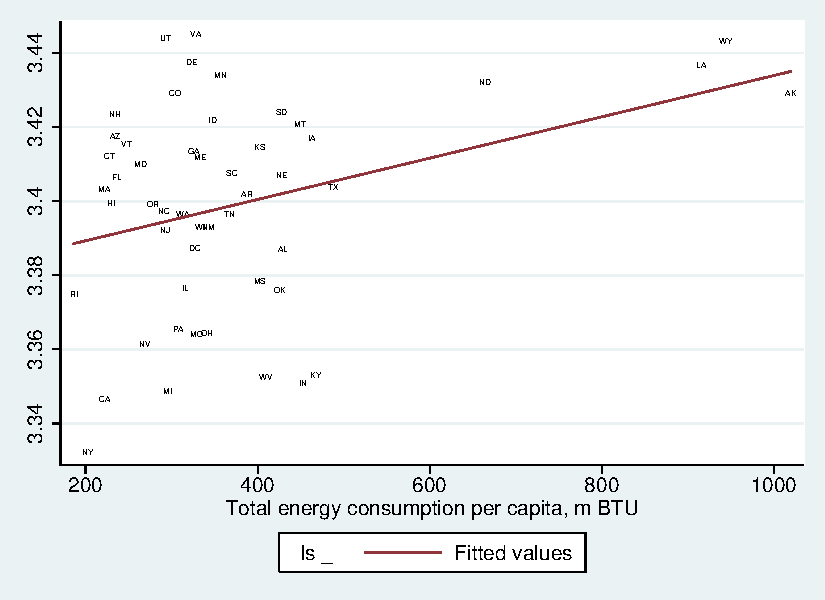
\includegraphics[height=3in]{/tmp/ls_en/lfTETPBls.pdf}\centering
\caption{lfTETPBls}\label{lfTETPBls}
\end{figure}


 We 
expect the  more dense and more urban areas are less happy. Note that ppulation
density and percent urban are very different variables--population density is
largely driven by history-when state was established--Western States (except
California) are less dense than North Eestern states. It is also driven by  size
of state--large states like Pennsylvania are less dense than smaller states like
Rhode Island. Percent urban is different--and it reflects administrative
prcesses such as zoning and is sensitive to a defninition of urban area. There are large differences in both
variables. In some North Eastern states there are more than 1,000 people per
square mile (NJ, RI), in most Western states, on the other hand, there are fewer
than 100 people per square mile. Several states are above 90\% urban, yet few
states are mostly non urban. Below a table sorted on population density.

Finally, we will look at 2 key variables for happiness, social support, one
measure of social capital, and the other ``harder'' measure--general
health. States in West and North are more supportive with an exception of
Delaware, which is very supportive and surrounded by unsupportive states.


\begin{spacing}{.8}
{\footnotesize
\begin{verbatim}
  | state     popDen   perUrb |  .  +---------------------+ 
  |---------------------------|     | state   supp     gh | 
  |    AK   .0012512    66.02 |     |---------------------| 
  |    WY   .0058089    64.76 |     |    HI   4.03   3.52 | 
  |    MT   .0068089    55.89 |     |    NY   4.05   3.60 | 
  |    ND    .009768     59.9 |     |    CA   4.09   3.53 | 
  |    SD   .0107636    56.65 |     |    DC   4.10   3.72 | 
  |---------------------------|     |    TX   4.11   3.46 | 
  |    NM   .0170242    77.43 |     |---------------------| 
  |    ID   .0190094    70.58 |     |    MS   4.11   3.30 | 
  |    NE   .0238206    73.13 |     |    AZ   4.13   3.57 | 
  |    NV   .0246217     94.2 |     |    CT   4.15   3.71 | 
  |    UT   .0337594    90.58 |     |    PA   4.15   3.55 | 
  |---------------------------|     |    FL   4.16   3.52 | 
  |    KS   .0349687     74.2 |     |---------------------| 
  |    OR   .0399737    81.03 |     |    MI   4.17   3.53 | 
  |    ME   .0430245    38.66 |     |    SC   4.18   3.47 | 
  |    CO   .0487062    86.15 |     |    NV   4.18   3.51 | 
  |    IA   .0546036    64.02 |     |    RI   4.19   3.64 | 
  |---------------------------|     |    IN   4.19   3.48 | 
  |    OK      .0548    66.24 |     |---------------------| 
  |    AR    .056154    56.16 |     |    KY   4.20   3.35 | 
  |    AZ   .0564202    89.81 |     |    MO   4.20   3.48 | 
  |    MS   .0632948    49.35 |     |    NM   4.21   3.51 | 
  |    MN   .0666861    73.27 |     |    AR   4.21   3.42 | 
  |---------------------------|     |    MT   4.21   3.59 | 
  |    VT   .0679205     38.9 |     |---------------------| 
  |    WV   .0771272    48.72 |     |    OH   4.21   3.51 | 
  |    MO   .0872253    70.44 |     |    IL   4.21   3.53 | 
  |    AL   .0945003    59.04 |     |    NE   4.22   3.61 | 
  |    TX   .0966383     84.7 |     |    AL   4.22   3.34 | 
  |---------------------------|     |    NH   4.22   3.69 | 
  |    WA   .1014513    84.05 |     |---------------------| 
  |    WI   .1050449    70.15 |     |    NJ   4.22   3.61 | 
  |    LA   .1051988    73.19 |     |    OR   4.23   3.58 | 
  |    KY    .110114    58.38 |     |    CO   4.23   3.69 | 
  |    NH   .1471073     60.3 |     |    NC   4.23   3.47 | 
  |---------------------------|     |    WA   4.24   3.59 | 
  |    TN   .1541655    66.39 |     |---------------------| 
  |    SC   .1542213    66.33 |     |    ME   4.24   3.60 | 
  |    GA   .1688821    75.07 |     |    SD   4.25   3.64 | 
  |    MI   .1746762    74.57 |     |    VT   4.25   3.74 | 
  |    IN   .1811528    72.44 |     |    ID   4.25   3.57 | 
  |---------------------------|     |    OK   4.25   3.38 | 
  |    NC   .1966354    66.09 |     |---------------------| 
  |    VA   .2031902    75.45 |     |    MA   4.26   3.74 | 
  |    HI   .2123741    91.93 |     |    MD   4.26   3.63 | 
  |    IL   .2312725    88.49 |     |    VA   4.27   3.63 | 
  |    CA   .2396597    94.95 |     |    LA   4.27   3.40 | 
  |---------------------------|     |    WY   4.27   3.63 | 
  |    OH   .2825454    77.92 |     |---------------------| 
  |    PA   .2840687    78.66 |     |    KS   4.27   3.60 | 
  |    FL   .3514421    91.16 |     |    GA   4.28   3.54 | 
  |    NY   .4116164    87.87 |     |    WI   4.28   3.61 | 
  |    DE   .4618843     83.3 |     |    AK   4.28   3.64 | 
  |---------------------------|     |    UT   4.29   3.71 | 
  |    MD    .596153     87.2 |     |---------------------| 
  |    CT   .7391024    87.99 |     |    IA   4.29   3.60 | 
  |    MA   .8414038    91.97 |     |    ND   4.30   3.59 | 
  |    RI   1.018562    90.73 |     |    WV   4.30   3.26 | 
  |    NJ      1.197    94.68 |     |    MN   4.31   3.72 | 
  |---------------------------|     |    DE   4.31   3.62 | 
  |    DC          .      100 |     |---------------------| 
  +---------------------------+     |    TN   4.32   3.42 | 
\end{verbatim}                      +---------------------+ 
}
\end{spacing}


Below regressions follow.  We have
seen that there is a weak to modearte relationshipe between energy use per
capita in different sectors and in general and happiness. How do these
relationships hold in regrressions? We proceed in a following way. We look at
three major energy uses: residential, commericial ,and transport  and also
total. We leave off indusrtial hence this energy is less liekly to impact
werllbeing of people directly and it may bias it--because this energy use is
dicatted by industry--there may be indiorect effects--thourgh employment, wages
adn development, but that shoudl be picked up by GDP. 
First, we
consider a model where we control for level of economic development (per capita
incoime). Then we add envioronmental factors, density, percent urban and avergae
temoertaures in Jan and Jul follwoning \citet{abdallah08al, brereton08}--we use
average for each month Jun and Jul and not the single max day. Finally, and this
is perhaps innovation in ecological literature, we add at state level two
aggregated from BRFSS key person level prodictors of happiness--social support
and happiness--tehre is substantail variation on these variables as discussed earlier.

We do not control for crime that is distributed unevenly within each state, and
hence global control in not informative.  

Let's start with residential energy, TERPB.
In column 1, relationship is positive  However, once controlling in column 2 for
population density and percent urban and tempoeratures , the relationship
between TERPB and happiness disappears. Likewise, when added in column 3
controls for social support and general health, the raltionship stays
non-existent. 


In transportation (TEAPB), on the other hand, the relationship is
positive, and if anything it increases with added controls, which is
puzzling. There are at least 2 explanations--perhaps thrill of travel %TODO cite
                                %from my ls_car paper  
Also, Americans prefer \citep{fuguitt90,fuguitt75} and are happier
\citep{aok_hea_spr,aok11a} in suburbs than in big cities, and there are likely
to be more consumption of energyu  in ransportatin in states woith more suburbs.
Likewise, when considering total energy use (TETPB) a positive relationship
persists. This warrants further exploration. 

\begin{table}[H]\centering \caption{ols1} \label{ols1} \begin{scriptsize} \begin{tabular}{p{1.4in}p{.43in}p{.43in}p{.43in}p{.43in}p{.43in}p{.43in}p{.43in}p{.43in}p{.43in}p{.43 in}p{.43in}p{.43 in}}\hline                     &      TERPB1   &      TERPB2   &      TERPB3   &      TEAPB1   &      TEAPB2   &      TEAPB3   &      TETPB1   &      TETPB2   &      TETPB3   \\
Total energy consumption per capita in the residential sector, m BTU&       0.000+  &       0.000   &       0.000   &               &               &               &               &               &               \\
Total energy consumption per capita in the transportation sector, m BTU&               &               &               &       0.000***&       0.000** &       0.000***&               &               &               \\
Total energy consumption per capita, m BTU&               &               &               &               &               &               &       0.000***&       0.000+  &       0.000***\\
Real gross domestic product, m chain 05usd, PC&       0.000+  &       0.002***&       0.001***&       0.000*  &       0.002***&       0.000+  &       0.000   &       0.002***&       0.000   \\
popukation density, thosands per sq m&               &      -0.029***&      -0.023***&               &      -0.022** &      -0.012** &               &      -0.024** &      -0.012*  \\
perUrb              &               &      -0.001***&      -0.001***&               &      -0.000** &      -0.000***&               &      -0.001** &      -0.000***\\
avgJanTemp          &               &      -0.000   &       0.001***&               &      -0.000   &       0.001***&               &      -0.000   &       0.001***\\
avgJulTemp          &               &       0.001*  &       0.002***&               &       0.001*  &       0.002***&               &       0.001*  &       0.002***\\
gh                 &               &               &       0.204***&               &               &       0.221***&               &               &       0.233***\\
supp               &               &               &       0.203***&               &               &       0.201***&               &               &       0.191***\\
constant            &       3.368***&       3.261***&       1.654***&       3.369***&       3.256***&       1.605***&       3.373***&       3.263***&       1.616***\\
N                   &         306   &         288   &         288   &         306   &         288   &         288   &         306   &         288   &         288   \\
 \hline\multicolumn{6}{l}{+p$<$0.10 *p$<$0.05 **p$<$0.01 ***p$<$0.001; robust standard errors} \end{tabular}\end{scriptsize}\end{table}


First considering enrgy use in residential and in commerce (columns a),
interestingly it appears that the positive relationship is driven by commerce,
residential energyu use indeed  turns negative. Then in columns b, when
considering all, three, residential, commerce, and transportation, thw first two
remain insignificant and transportation coomes out positive


\begin{table}[H]\centering \caption{ols2} \label{ols2} \begin{scriptsize} \begin{tabular}{p{1.4in}p{.43in}p{.43in}p{.43in}p{.43in}p{.43in}p{.43in}p{.43in}p{.43in}p{.43in}p{.43 in}p{.43in}p{.43 in}}\hline                     &          a1   &          a2   &          a3   &          b1   &          b2   &          b3   \\
Total energy consumption per capita in the residential sector, m BTU&       0.000   &      -0.000   &      -0.000+  &       0.000   &      -0.000   &      -0.000   \\
Total energy consumption per capita in the transportation sector, m BTU&               &               &               &       0.000***&       0.000   &       0.000***\\
TET*                &               &               &               &               &               &               \\
Total energy consumption per capita in the commercial sector, m BTU&       0.000   &       0.001***&       0.001***&      -0.000   &       0.000   &      -0.000   \\
Real gross domestic product, m chain 05usd, PC&       0.000   &       0.002***&       0.000*  &       0.000   &       0.002***&       0.000+  \\
popukation density, thosands per sq m&               &      -0.023** &      -0.018***&               &      -0.022** &      -0.012** \\
perUrb              &               &      -0.001***&      -0.001***&               &      -0.001** &      -0.000** \\
avgJanTemp          &               &      -0.000   &       0.001***&               &      -0.000   &       0.001***\\
avgJulTemp          &               &       0.001*  &       0.002***&               &       0.001*  &       0.002***\\
gh                 &               &               &       0.201***&               &               &       0.218***\\
supp               &               &               &       0.208***&               &               &       0.204***\\
constant            &       3.374***&       3.280***&       1.665***&       3.350***&       3.276***&       1.603***\\
N                   &         306   &         288   &         288   &         306   &         288   &         288   \\
 \hline\multicolumn{6}{l}{+p$<$0.10 *p$<$0.05 **p$<$0.01 ***p$<$0.001; robust standard errors} \end{tabular}\end{scriptsize}\end{table}

These findings are lagrly replicated with fixed effects estimatiion--there is no
increase in happiness from energy use in residential or total, but tehre is an
increase in transportation. Note, hausman test indicates that we should use
fixed, not random effect.  


\begin{table}[H]\centering \caption{fe1} \label{fe1} \begin{scriptsize} \begin{tabular}{p{1.4in}p{.43in}p{.43in}p{.43in}p{.43in}p{.43in}p{.43in}p{.43in}p{.43in}p{.43in}p{.43 in}p{.43in}p{.43 in}}\hline                     &      TERPB1   &      TERPB2   &      TERPB3   &      TEAPB1   &      TEAPB2   &      TEAPB3   &      TETPB1   &      TETPB2   &      TETPB3   \\
Total energy consumption per capita in the residential sector, m BTU&      -0.001+  &      -0.001   &      -0.000   &               &               &               &               &               &               \\
Total energy consumption per capita in the transportation sector, m BTU&               &               &               &      -0.000+  &      -0.000   &       0.000+  &               &               &               \\
Total energy consumption per capita, m BTU&               &               &               &               &               &               &      -0.000   &       0.000   &       0.000   \\
Real gross domestic product, m chain 05usd, PC&       0.003***&       0.003***&       0.003***&       0.003***&       0.003** &       0.002** &       0.003***&       0.002*  &       0.002** \\
popukation density, thosands per sq m&               &       0.456   &       0.027   &               &       0.532   &       0.175   &               &       0.687+  &       0.135   \\
perUrb              &               &       0.011***&       0.008** &               &       0.011***&       0.008** &               &       0.011***&       0.008** \\
avgJanTemp          &               &       0.000   &       0.000   &               &       0.000+  &       0.000   &               &       0.001*  &       0.000   \\
avgJulTemp          &               &       0.003***&       0.002***&               &       0.002***&       0.001** &               &       0.002***&       0.002***\\
gh                 &               &               &       0.212***&               &               &       0.220***&               &               &       0.212***\\
supp               &               &               &       0.162***&               &               &       0.168***&               &               &       0.161***\\
constant            &       3.307***&       2.211***&       1.168***&       3.288***&       2.193***&       1.033***&       3.285***&       2.140***&       1.134***\\
N                   &         306   &         288   &         288   &         306   &         288   &         288   &         306   &         288   &         288   \\
 \hline\multicolumn{6}{l}{+p$<$0.10 *p$<$0.05 **p$<$0.01 ***p$<$0.001; robust standard errors} \end{tabular}\end{scriptsize}\end{table}


%TODO defineitly have beta coeff some hwere--see what ecological econ
%doeas--maybe in app if they don;t do that a lot..

\section{Counties}

\begin{figure}[H]
 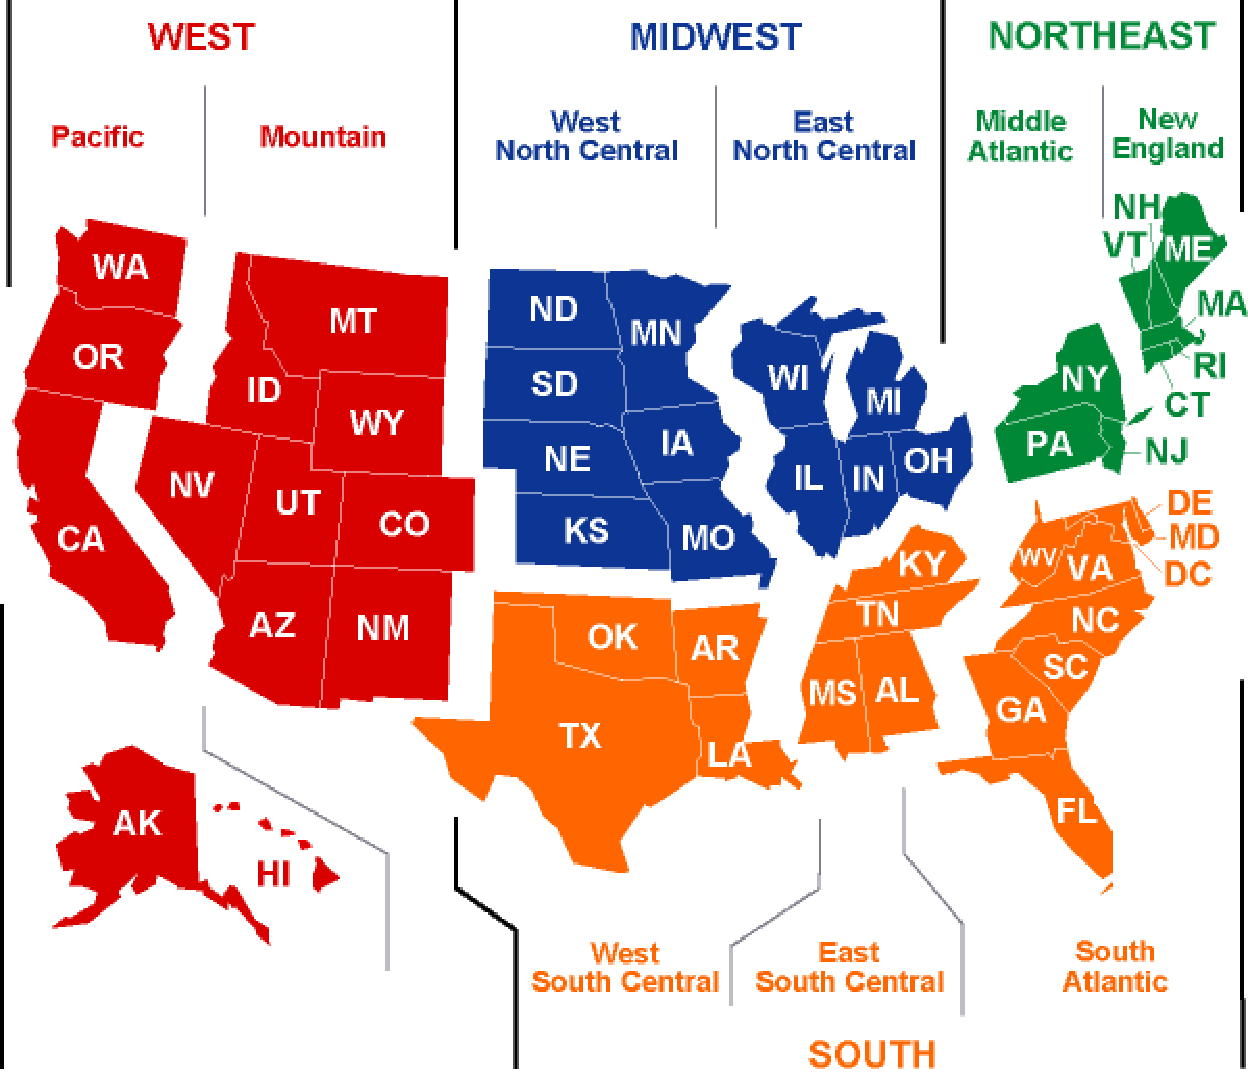
\includegraphics[height=3in]{/home/aok/papers/lonnie_issp_work/tex/cendivco.pdf}\centering
\caption{California climate divisions correspondencies with California
  counties. \url{http://www.cpc.ncep.noaa.gov/products/analysis_monitoring/regional_monitoring/CLIM_DIVS/california.gif}.}\label{caCD}
\end{figure}

Note, as shown in figure \ref{caCD}, there is not always an exact overlap
between counties and climate divisions. They were matched in the following way

The limitation of states is that, well, it is very ecological--large areas! and
second, there is not much difference is happijess ascross states, buit there is
much more across counties. 

Here in bivariate case, too, like across states, there is a positive
relationshipe between energy consumprion and happiness, yet it is somewhat
weaker. 

\begin{figure}[H]
 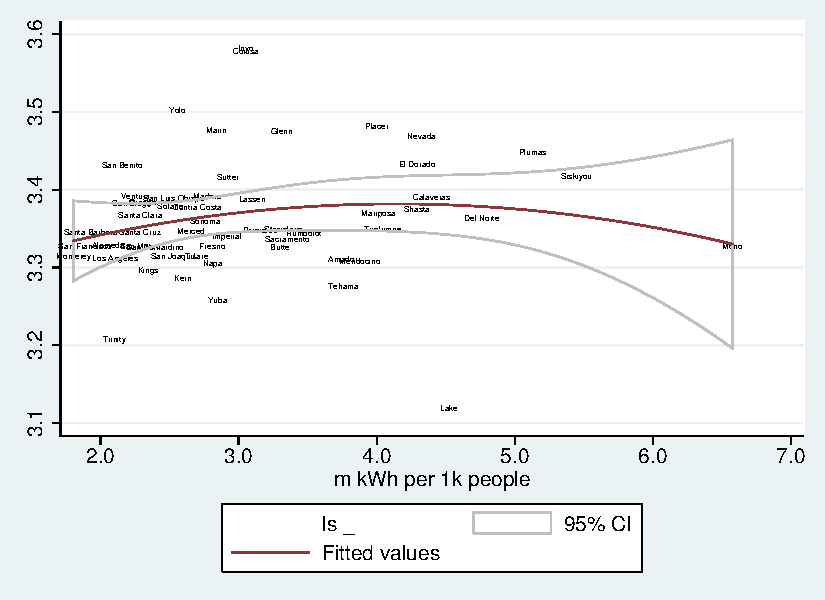
\includegraphics[height=3in]{/tmp/ls_en/lfELERESls.pdf}\centering
\caption{lfELERESls}\label{lfELERESls}
\end{figure}

\begin{figure}[H]
 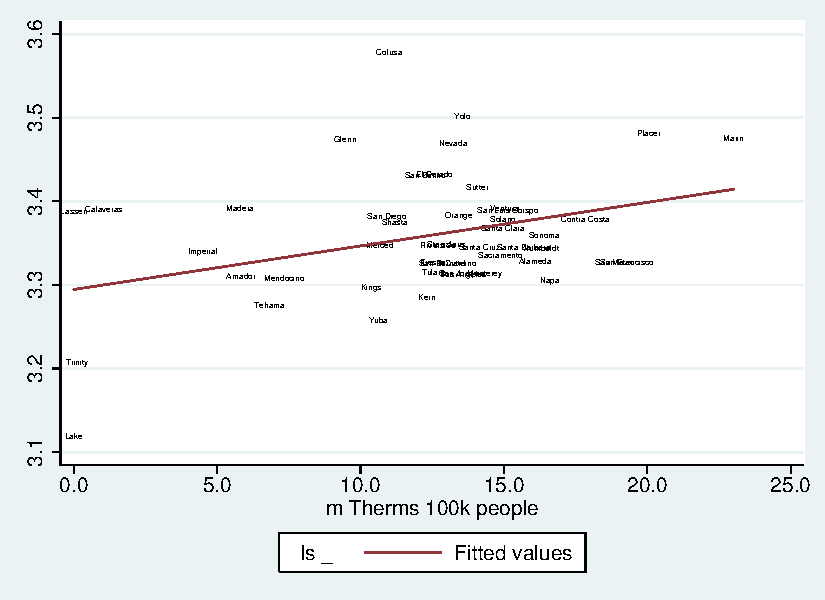
\includegraphics[height=3in]{/tmp/ls_en/lfGASls.pdf}\centering
\caption{lfGASls}\label{lfGASls}
\end{figure}



\begin{spacing}{.8}
{\footnotesize
\begin{verbatim}
SORTED OON ELERES
  ----------------------------------+
           county   eleres   eletot |
  ----------------------------------|
          Trinity      0.8      8.1 |
         Monterey      1.8      5.9 |
             Inyo      1.9      4.5 |
    Santa Barbara      1.9      7.5 |
    San Francisco      1.9      7.3 |
  ----------------------------------|
      Los Angeles      2.0      6.8 |
          Alameda      2.0      7.2 |
       San Benito      2.1      5.6 |
        San Diego      2.1      6.1 |
          Ventura      2.1      6.5 |
  ----------------------------------|
      Santa Clara      2.2      9.3 |
   San Bernardino      2.2      6.5 |
        San Mateo      2.3      6.6 |
            Kings      2.3      9.7 |
           Orange      2.3      6.9 |
  ----------------------------------|
       Santa Cruz      2.3      4.8 |
           Solano      2.4      7.5 |
  San Luis Obispo      2.4      6.1 |
      San Joaquin      2.4      8.1 |
             Yolo      2.5      8.2 |
  ----------------------------------|
             Kern      2.5     17.7 |
           Tulare      2.5      8.5 |
           Merced      2.6     14.1 |
     Contra Costa      2.6      8.8 |
           Madera      2.7      9.1 |
  ----------------------------------|
           Fresno      2.7      7.5 |
             Napa      2.8      7.5 |
            Marin      2.8      5.6 |
           Sonoma      2.8      5.9 |
           Sutter      2.8      6.3 |
  ----------------------------------|
             Yuba      2.8      6.7 |
        Riverside      2.8      6.2 |
         Imperial      2.8      8.0 |
           Colusa      3.0     12.0 |
           Lassen      3.0     11.5 |
  ----------------------------------|
       Stanislaus      3.2      8.9 |
       Sacramento      3.2      7.5 |
            Glenn      3.3     10.7 |
            Butte      3.3      6.5 |
         Humboldt      3.6      6.8 |
  ----------------------------------|
           Tehama      3.7      7.8 |
           Amador      3.7      8.4 |
           Placer      3.8      8.4 |
        Mendocino      3.9      6.8 |
         Mariposa      4.0      6.2 |
  ----------------------------------|
         Tuolumne      4.1      8.1 |
           Shasta      4.2      8.8 |
        El Dorado      4.2      6.9 |
           Nevada      4.3      6.7 |
        Calaveras      4.4      7.1 |
  ----------------------------------|
             Lake      4.6      7.0 |
        Del Norte      4.8      8.1 |
           Plumas      5.2     10.2 |
         Siskiyou      5.4     11.2 |
             Mono      6.6     14.5 |
  ----------------------------------|
           Alpine        .        . |
           Sierra        .        . |
            Modoc        .        . |
  				   
  ----------------------------------+

SORTED ON GASRES

           county   gasres   gastot |
  ----------------------------------|
             Lake      0.0      0.0 |
           Lassen      0.0      0.0 |
          Trinity      0.2      0.5 |
        Calaveras      1.0      2.0 |
         Imperial      4.4     17.6 |
  ----------------------------------|
           Madera      5.8     28.3 |
           Amador      5.8     24.1 |
           Tehama      6.9     17.3 |
        Mendocino      7.3     12.1 |
            Glenn      9.5     27.6 |
  ----------------------------------|
            Kings     10.2     44.9 |
           Merced     10.6     45.3 |
             Yuba     10.7     16.6 |
        San Diego     10.9     18.1 |
           Colusa     11.1    121.9 |
  ----------------------------------|
           Shasta     11.4     19.2 |
        Riverside     12.1     18.3 |
             Kern     12.1    276.3 |
       San Benito     12.2     23.7 |
           Fresno     12.3     30.3 |
  ----------------------------------|
           Tulare     12.4     35.3 |
        El Dorado     12.7     17.3 |
       Stanislaus     12.9     33.6 |
   San Bernardino     13.2     24.1 |
           Orange     13.4     21.2 |
  ----------------------------------|
           Nevada     13.4     19.1 |
            Butte     13.4     21.6 |
             Yolo     13.5     30.9 |
      San Joaquin     13.5     28.9 |
           Sutter     13.8     22.7 |
  ----------------------------------|
      Los Angeles     13.8     31.8 |
         Monterey     13.9     26.0 |
       Santa Cruz     13.9     21.9 |
      Santa Clara     14.5     25.6 |
       Sacramento     14.8     22.2 |
  ----------------------------------|
          Ventura     14.9     24.3 |
  San Luis Obispo     15.0     29.3 |
           Solano     15.1     54.6 |
    Santa Barbara     15.5     29.9 |
         Humboldt     15.7     24.7 |
  ----------------------------------|
          Alameda     15.8     27.7 |
           Sonoma     16.0     23.7 |
             Napa     16.6     29.2 |
           Placer     17.6     26.1 |
     Contra Costa     17.8     96.4 |
  ----------------------------------|
        San Mateo     18.4     30.7 |
    San Francisco     19.0     32.7 |
            Marin     22.6     31.4 |
            Modoc        .        . |
           Alpine        .        . |
  ----------------------------------|
        Del Norte        .        . |
         Siskiyou        .        . |
             Inyo        .        . |
           Plumas        .        . |
             Mono        .        . |
  ----------------------------------|
           Sierra        .        . |
         Mariposa        .        . |
         Tuolumne        .        . |
  ----------------------------------+

\end{verbatim}
}
\end{spacing}


And now regressions. Natural gas usage is a function of its availabily, not
necassarily gas hunger--for instance Lassen County has zero natural gas
use. Furthermore if gas is unused then it may be compensated with other sources,
hence electricty and gas in one regression. And as expected, no effect in
happiness. 

\begin{table}[H]\centering \caption{CAols1} \label{CAols1} \begin{scriptsize} \begin{tabular}{p{1.4in}p{.43in}p{.43in}p{.43in}p{.43in}p{.43in}p{.43in}p{.43in}p{.43in}p{.43in}p{.43 in}p{.43in}p{.43 in}}\hline                     &     eleres1   &     eleres2   &     eleres3   &     eletot1   &     eletot2   &     eletot3   &     gasres1   &     gasres2   &     gasres3   &     gastot1   &     gastot2   &     gastot3   \\
m kWh per 1k people &       0.020   &       0.023   &       0.009   &               &               &               &       0.041** &       0.041*  &       0.016   &               &               &               \\
per capita personal income&       0.000** &       0.000***&       0.000   &       0.000*  &       0.000** &       0.000   &       0.000   &       0.000   &      -0.000   &       0.000***&       0.000***&       0.000   \\
popDen              &               &      -0.000*  &      -0.000   &               &      -0.000** &      -0.000   &               &      -0.000+  &      -0.000   &               &      -0.000** &      -0.000   \\
avgJanTemp          &               &       0.001   &       0.002   &               &      -0.001   &       0.002   &               &       0.001   &       0.002   &               &      -0.002   &       0.002   \\
avgJulTemp          &               &       0.003   &       0.003   &               &       0.003   &       0.003   &               &      -0.000   &       0.001   &               &       0.002   &       0.001   \\
gh                 &               &               &       0.135*  &               &               &       0.146** &               &               &       0.105+  &               &               &       0.134*  \\
supp               &               &               &       0.183*  &               &               &       0.185*  &               &               &       0.194*  &               &               &       0.195*  \\
m kWh per 1k people &               &               &               &       0.001   &       0.001   &       0.002   &               &               &               &       0.007   &       0.006   &       0.005   \\
m Therms 100k people&               &               &               &               &               &               &       0.005   &       0.005   &       0.004   &               &               &               \\
m Therms 100k people&               &               &               &               &               &               &               &               &               &      -0.000   &      -0.000   &      -0.000   \\
constant            &       3.227***&       2.916***&       1.773***&       3.294***&       3.085***&       1.764***&       3.134***&       3.092***&       1.966***&       3.229***&       3.160***&       1.825***\\
N                   &         219   &         219   &         219   &         219   &         219   &         219   &         198   &         198   &         198   &         198   &         198   &         198   \\
 \hline\multicolumn{6}{l}{+p$<$0.10 *p$<$0.05 **p$<$0.01 ***p$<$0.001; robust standard errors} \end{tabular}\end{scriptsize}\end{table}


and in table \ref{CAfe1} a bit of bummer --elecricity residential appears to
have effect on happiness if in fixed effects model adn together with natural gas:(
\begin{table}[H]\centering \caption{CAfe1} \label{CAfe1} \begin{scriptsize} \begin{tabular}{p{1.4in}p{.43in}p{.43in}p{.43in}p{.43in}p{.43in}p{.43in}p{.43in}p{.43in}p{.43in}p{.43 in}p{.43in}p{.43 in}}\hline                     &     eleres1   &     eleres2   &     eleres3   &     gasres1   &     gasres2   &     gasres3   \\
m kWh per 1k people &       0.053*  &       0.062*  &       0.037   &       0.154***&       0.164***&       0.149***\\
per capita personal income&      -0.000   &       0.000   &       0.000   &      -0.000   &       0.000   &       0.000   \\
popDen              &               &      -0.000   &       0.000   &               &      -0.000   &      -0.000   \\
avgJanTemp          &               &       0.005   &       0.005   &               &       0.005   &       0.006+  \\
avgJulTemp          &               &       0.001   &       0.006   &               &      -0.001   &       0.001   \\
gh                 &               &               &       0.175** &               &               &       0.177***\\
supp               &               &               &       0.148** &               &               &       0.067   \\
m Therms 100k people&               &               &               &      -0.007   &      -0.004   &       0.005   \\
constant            &       3.363***&       2.975***&       1.322+  &       3.056***&       2.799***&       1.533*  \\
N                   &         219   &         219   &         219   &         198   &         198   &         198   \\
 \hline\multicolumn{6}{l}{+p$<$0.10 *p$<$0.05 **p$<$0.01 ***p$<$0.001; robust standard errors} \end{tabular}\end{scriptsize}\end{table}


\section{Counties--SMART version}

A limitation of BRFSS data at county level is that it is not representatoibe of
counties. And there are likely problems--for instamce Mono county increased
happiness from 2.82 in 2008 to 3.62, which is an extermely large increase and
likely due to sampling. To perform a robustness check whether these results may
 be due to sampling, we have rerun m,odels using SMART verion of data that is
 represnetative of counties

!!TODO!!  


\begin{verbatim}

\end{verbatim}


\newpage
\bibliography{/home/aok/papers/root/tex/ebib.bib}

\end{spacing}
\end{document}
